\documentclass[11pt,a4paper]{article}

\usepackage[T1]{fontenc}
\usepackage[utf8]{inputenc}
\usepackage[margin=1in]{geometry}
\usepackage{amsmath,amssymb}
\usepackage{graphicx}
\usepackage{booktabs}
\usepackage{caption}
\usepackage{subcaption}
\usepackage{xcolor}
\usepackage[colorlinks=true,linkcolor=blue!50!black,urlcolor=blue!50!black]{hyperref}

\captionsetup{font=small,labelfont=bf}
\newcommand{\code}[1]{\texttt{#1}}

\title{Assignment 2 Report:\\Halfedge Mesh Traversal, Edge Flips, and Subdivision}
\author{Naufal Zafran Fadil\\[2pt]\small NPM 2406402542\\[2pt]\small CSCE604029 Computer Graphics, Universitas Indonesia}
\date{October 2026}

\begin{document}
\maketitle

\begin{abstract}
This report accompanies the halfedge mesh implementation (traversal, face
geometry, mesh summary, edge flip, linear and Catmull--Clark subdivision).
Section~1 describes the checks and gives mesh summaries before and after one
subdivision step, Section~2 reports edge-flip acceptance and rejection, and
Section~3 compares one to four steps of both subdivision schemes on the cube.
\end{abstract}

\section{Checks and mesh summaries}
All six unit-test groups pass. They check traversal on every provided mesh,
boundary circulation, rotated face starts, normals and areas (including the
L-shaped cap of area 8), rejected flips without mutation, double-flip reversal,
and subdivision connectivity, vertex order, positions, and input immutability.
The cube is also checked through four levels of each subdivision scheme.

\textbf{Command:} \code{python -m unittest -v test\_student}

\begin{table}[ht]
\centering
\caption{Every provided mesh before and after one applicable subdivision step.
  Generated by \code{python report\_data.py}. $\chi=V-E+F$ counts interior faces.}
\vspace{3pt}
\small
\begin{tabular}{llrrrrr}
\toprule
Mesh & Scheme & $V$ & $E$ & $F$ & $\chi$ & Area \\
\midrule
cube & input & 8 & 12 & 6 & 2 & 24.000 \\
cube & linear & 26 & 48 & 24 & 2 & 24.000 \\
cube & Catmull--Clark & 26 & 48 & 24 & 2 & 11.528 \\
fan & input & 7 & 12 & 6 & 1 & 2.750 \\
fan & linear & 25 & 42 & 18 & 1 & 2.750 \\
grid & input & 16 & 24 & 9 & 1 & 9.125 \\
grid & linear & 49 & 84 & 36 & 1 & 9.112 \\
lshape & input & 12 & 18 & 8 & 2 & 23.200 \\
lshape & linear & 38 & 72 & 36 & 2 & 23.200 \\
lshape & Catmull--Clark & 38 & 72 & 36 & 2 & 14.106 \\
octahedron & input & 6 & 12 & 8 & 2 & 6.928 \\
octahedron & linear & 26 & 48 & 24 & 2 & 6.928 \\
octahedron & Catmull--Clark & 26 & 48 & 24 & 2 & 3.775 \\
pyramid & input & 5 & 8 & 5 & 2 & 11.211 \\
pyramid & linear & 18 & 32 & 16 & 2 & 11.211 \\
pyramid & Catmull--Clark & 18 & 32 & 16 & 2 & 3.903 \\
tetrahedron & input & 4 & 6 & 4 & 2 & 13.856 \\
tetrahedron & linear & 14 & 24 & 12 & 2 & 13.856 \\
tetrahedron & Catmull--Clark & 14 & 24 & 12 & 2 & 3.430 \\
torus & input & 72 & 144 & 72 & 0 & 12.823 \\
torus & linear & 288 & 576 & 288 & 0 & 12.823 \\
torus & Catmull--Clark & 288 & 576 & 288 & 0 & 11.219 \\
\bottomrule
\end{tabular}
\end{table}

Each old edge adds one vertex and each old face adds one vertex, so
$V'=V+E+F$. Each face corner becomes one quad, giving
$F'=\sum_f\deg(f)$. Splitting each original edge contributes $2E$ edges;
connecting each face point to its surrounding edge points contributes $F'$,
so $E'=2E+F'$. Consequently $V'-E'+F'=V-E+F$, matching the table for both
open and closed meshes.

\section{Edge flip acceptance and rejection}
Each edge index was tried independently on a freshly loaded mesh. Every
accepted flip passed \code{mesh.validate()}, and a second flip restored each
halfedge's original twin, next, target, edge, and face links. Every rejected
flip left those links unchanged.

\textbf{Commands:} \code{python report\_data.py};
\code{python -m unittest -v test\_student}

\begin{table}[ht]
\centering
\caption{Independent attempts on every edge. Counts come from
  \code{python report\_data.py}.}
\vspace{3pt}
\small
\begin{tabular}{lrrrrr}
\toprule
Mesh & Edges & Accepted & Boundary & Nontriangle & Already joined \\
\midrule
octahedron & 12 & 12 & 0 & 0 & 0 \\
fan & 12 & 6 & 6 & 0 & 0 \\
pyramid & 8 & 4 & 0 & 4 & 0 \\
tetrahedron & 6 & 0 & 0 & 0 & 6 \\
\bottomrule
\end{tabular}
\end{table}

\paragraph{Boundary edge.} There is no second interior triangle. Applying the
two-triangle rewiring would damage the boundary loop.

\paragraph{Nontriangle incident face.} The six-halfedge local pattern no longer
covers both face loops. Rewiring only those six halfedges would leave corners
or edges disconnected from the intended faces.

\paragraph{Opposite vertices already joined.} The new diagonal would duplicate
an existing edge, so two halfedges would run between the same ordered
vertices; \code{mesh.validate()} rejects that connectivity.

\begin{figure}[ht]
\centering
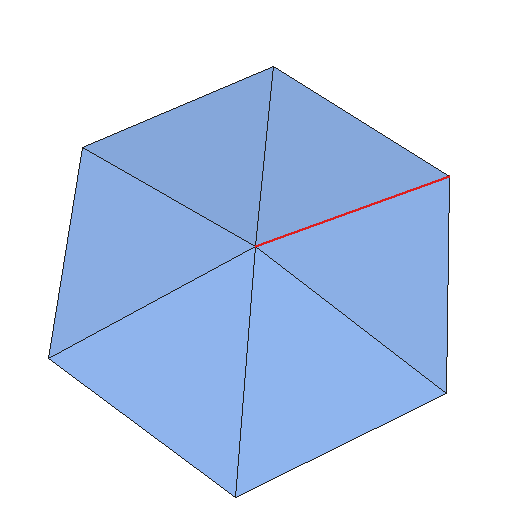
\includegraphics[width=0.40\textwidth]{figs/fan-before.png}\hfill
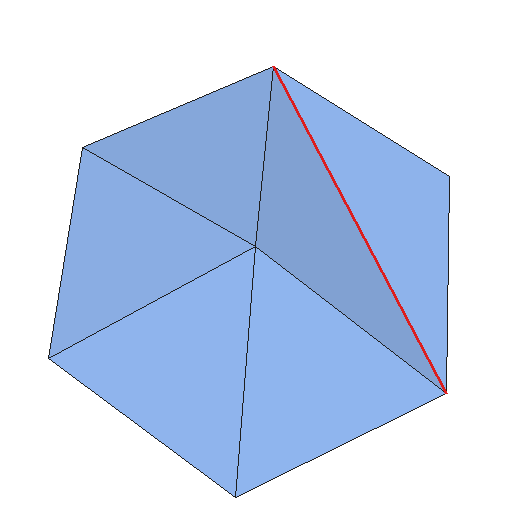
\includegraphics[width=0.40\textwidth]{figs/fan-after.png}
\caption{Fan edge 0 before (left) and after (right) its flip. The highlighted
diagonal changes endpoints while the boundary stays intact. Both images are
generated by \code{python report\_data.py}.}
\end{figure}

\section{Cube subdivision: one to four steps}
\textbf{Command:} \code{python report\_data.py} generates the counts, areas,
valences, and sample renders below.

\begin{table}[ht]
\centering
\caption{Cube face count, surface area, and number of vertices with valence
different from four after each step. Vertex counts are included for reference.}
\vspace{3pt}
\small
\begin{tabular}{rrrrrrr}
\toprule
Step & Faces & $V$ & Linear area & Linear non-4 & CC area & CC non-4 \\
\midrule
0 & 6 & 8 & 24.000000 & 8 & 24.000000 & 8 \\
1 & 24 & 26 & 24.000000 & 8 & 11.527744 & 8 \\
2 & 96 & 98 & 24.000000 & 8 & 9.727718 & 8 \\
3 & 384 & 386 & 24.000000 & 8 & 9.326891 & 8 \\
4 & 1536 & 1538 & 24.000000 & 8 & 9.229708 & 8 \\
\bottomrule
\end{tabular}
\end{table}

The schemes use identical quad connectivity, hence identical face and vertex
counts: $F_k=6\cdot4^k$ and $V_k=F_k+2$. The eight original cube corners retain
valence 3; newly inserted vertices have valence 4. Linear subdivision keeps
old vertices fixed and places new points on the cube's planar faces, so the
surface area remains 24. Catmull--Clark moves original and edge vertices
inward, rounding the cube; its area falls to 9.229708 by step 4.

\begin{figure}[ht]
\centering
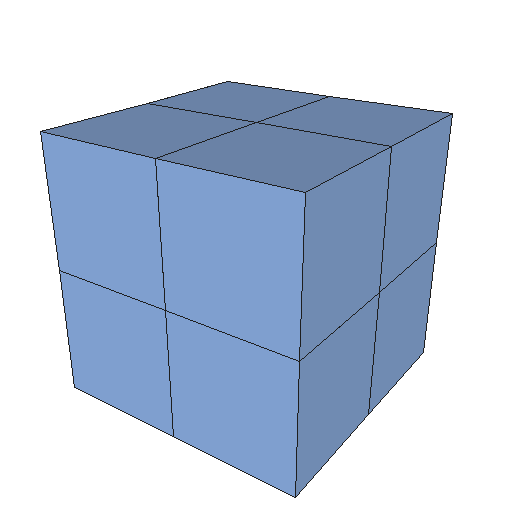
\includegraphics[width=0.36\textwidth]{figs/cube-linear-1.png}\hspace{0.08\textwidth}
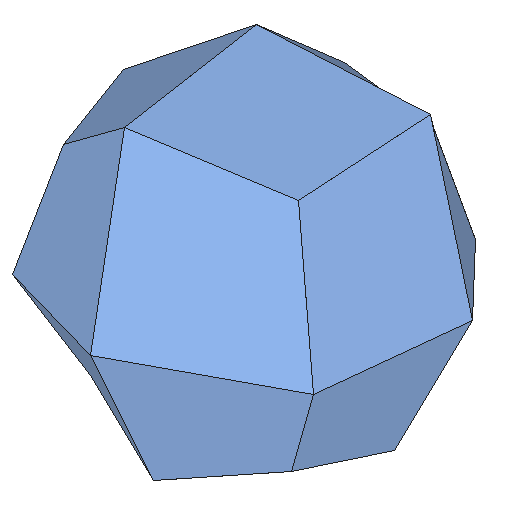
\includegraphics[width=0.36\textwidth]{figs/cube-catmull-clark-1.png}\\[3pt]
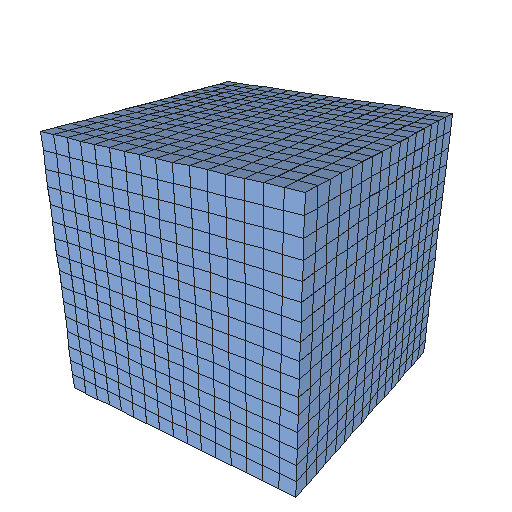
\includegraphics[width=0.36\textwidth]{figs/cube-linear-4.png}\hspace{0.08\textwidth}
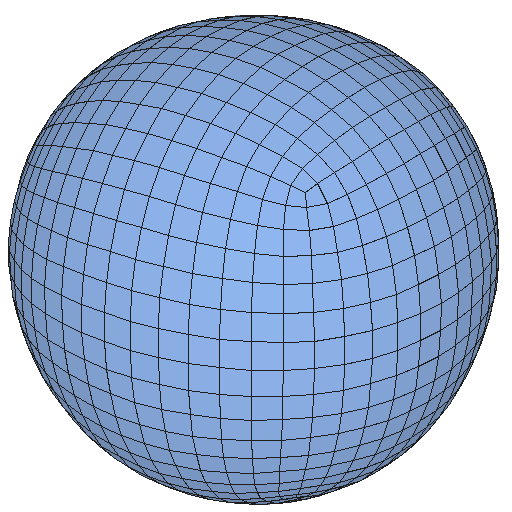
\includegraphics[width=0.36\textwidth]{figs/cube-catmull-clark-4.png}
\caption{Linear (left) and Catmull--Clark (right) on the cube at steps 1
(top) and 4 (bottom). Generated by \code{python report\_data.py}.}
\end{figure}

\end{document}
